\documentclass{beamer}

\pdfmapfile{+sansmathaccent.map}


\mode<presentation>
{
  \usetheme{Warsaw} % or try Darmstadt, Madrid, Warsaw, Rochester, CambridgeUS, ...
  \usecolortheme{seahorse} % or try seahorse, beaver, crane, wolverine, ...
  \usefonttheme{serif}  % or try serif, structurebold, ...
  \setbeamertemplate{navigation symbols}{}
  \setbeamertemplate{caption}[numbered]
} 


%%%%%%%%%%%%%%%%%%%%%%%%%%%%
% itemize settings

\definecolor{mypink}{RGB}{255, 150, 150}
\definecolor{myblue}{RGB}{150, 150, 255}
\definecolor{mygray}{gray}{0.8}

\setbeamertemplate{itemize items}[default]

\setbeamertemplate{itemize item}{\color{mypink}$\blacksquare$}
\setbeamertemplate{itemize subitem}{\color{myblue}$\blacktriangleright$}
\setbeamertemplate{itemize subsubitem}{\color{mygray}$\blacksquare$}

%%%%%%%%%%%%%%%%%%%%%%%%%%%%
% block settings

\setbeamercolor{block title}{bg=red!30,fg=black}


%%%%%%%%%%%%%%%%%%%%%%%%%%%%
% URL settings
\hypersetup{
    colorlinks=true,
    linkcolor=blue,
    filecolor=blue,      
    urlcolor=blue,
}

%%%%%%%%%%%%%%%%%%%%%%%%%%

\renewcommand{\familydefault}{\rmdefault}

\usepackage{amsmath}
\usepackage{mathtools}

\DeclareMathOperator*{\argmin}{arg\,min}

\usepackage{subcaption}




%%%%%%%%%%%%%%%%%%%%%%%%%%%%
% code settings

\usepackage{listings}
\usepackage{color}
\definecolor{mygreen}{rgb}{0,0.6,0}
\definecolor{mygray}{rgb}{0.5,0.5,0.5}
\definecolor{mymauve}{rgb}{0.58,0,0.82}
\lstset{ 
  backgroundcolor=\color{white},   % choose the background color; you must add \usepackage{color} or \usepackage{xcolor}; should come as last argument
  basicstyle=\footnotesize,        % the size of the fonts that are used for the code
  breakatwhitespace=false,         % sets if automatic breaks should only happen at whitespace
  breaklines=true,                 % sets automatic line breaking
  captionpos=b,                    % sets the caption-position to bottom
  commentstyle=\color{mygreen},    % comment style
  deletekeywords={...},            % if you want to delete keywords from the given language
  escapeinside={\%*}{*)},          % if you want to add LaTeX within your code
  extendedchars=true,              % lets you use non-ASCII characters; for 8-bits encodings only, does not work with UTF-8
  firstnumber=0000,                % start line enumeration with line 0000
  frame=single,	                   % adds a frame around the code
  keepspaces=true,                 % keeps spaces in text, useful for keeping indentation of code (possibly needs columns=flexible)
  keywordstyle=\color{blue},       % keyword style
  language=Octave,                 % the language of the code
  morekeywords={*,...},            % if you want to add more keywords to the set
  numbers=left,                    % where to put the line-numbers; possible values are (none, left, right)
  numbersep=5pt,                   % how far the line-numbers are from the code
  numberstyle=\tiny\color{mygray}, % the style that is used for the line-numbers
  rulecolor=\color{black},         % if not set, the frame-color may be changed on line-breaks within not-black text (e.g. comments (green here))
  showspaces=false,                % show spaces everywhere adding particular underscores; it overrides 'showstringspaces'
  showstringspaces=false,          % underline spaces within strings only
  showtabs=false,                  % show tabs within strings adding particular underscores
  stepnumber=2,                    % the step between two line-numbers. If it's 1, each line will be numbered
  stringstyle=\color{mymauve},     % string literal style
  tabsize=2,	                   % sets default tabsize to 2 spaces
  title=\lstname                   % show the filename of files included with \lstinputlisting; also try caption instead of title
}

%%%%%%%%%%%%%%%%%%%%%%%%%%%%
% tikz settings

\usepackage{tikz}
\tikzset{every picture/.style={line width=0.75pt}}


\title{Manipulator Equations for Systems with Constraints}
\subtitle{Contact-aware Control, Lecture 4}
\author{by Sergei Savin}
\centering
\date{Fall 2020}



\begin{document}
\maketitle


\begin{frame}{Content}

\begin{itemize}
\item Lagrange equations
\item Kinetic energy encoding (parts 1-4)
\item Generalized inertia
\begin{itemize}
\item Part 1-2
\item Part 3-4: Christoffel symbols
\item Part 5-6: Alternative formulation
\end{itemize}
\item Generalized forces
\begin{itemize}
\item Part 1, General case
\item Part 2, Conservative forces
\item Part 3-4, Reaction forces
\end{itemize}
\item Manipulator equations
\begin{itemize}
\item Part 1, no reaction forces
\item Part 2, reaction forces
\end{itemize}
\item Read more
\item Homework
\end{itemize}

\end{frame}



\begin{frame}{Lagrange equations}
% \framesubtitle{O}
\begin{flushleft}

Remember Lagrange equations:

\begin{equation}
\label{eq:Lagrange}
    \frac{d}{dt} \bigg( 
    \frac{\partial T }{\partial \dot{\bo{q}}}
    \bigg) - 
    \frac{\partial T }{\partial \bo{q}} = \tau
\end{equation}

Let us remember that in the general case of point masses, kinetic energy is:

\begin{equation}
\label{eq:kinetic_energy}
    T = \sum 0.5 m_i \dot{\bo{r}}_i^\top \dot{\bo{r}}_i,
\end{equation}

and in the general case of rigid bodies, it is:

\begin{equation}
\label{eq:kinetic_energy_rigid_body}
    T = \sum 0.5 m_i \dot{\bo{r}}_i^\top \dot{\bo{r}}_i + \sum 0.5 \bo{w}_i^\top \bo{I}_i \bo{w}_i,
\end{equation}

Where $\dot{\bo{r}}_i$ is the velocity of the center of mass of the $i$-th body, and $\bo{w}$ is the angular velocity of that body.

\end{flushleft}
\end{frame}




\begin{frame}{Kinetic energy encoding}
\framesubtitle{Part 1}
\begin{flushleft}

Using chain rule we can describe the velocity of the center of mass:

\begin{equation}
\dot{\bo{r}}_i = \frac{\partial \bo{r}_i }{\partial {\bo{q}}} \dot{\bo{q}} = \bo{J}^v_i \dot{\bo{q}}
\end{equation}

This establishes the connection between $\dot{\bo{r}}_i$ and generalized velocities.

\end{flushleft}
\end{frame}




\begin{frame}{Kinetic energy encoding}
\framesubtitle{Part 2}
\begin{flushleft}

For the rotations, it is not as simple. We start by using a Poisson formula to connect rotation matrix $\bo{T}(\bo{q})$ of a body to angular velocity of a body:

\begin{equation}
\bo{W}(\bo{q}, \dot{\bo{q}}) = \bo{T} \dot{\bo{T}}, \ \ \dot{\bo{T}}(\bo{q}, \dot{\bo{q}}) = \frac{\partial \bo{T}}{\partial {\bo{q}}} \dot{\bo{q}}
\end{equation}

where $\bo{W}(\bo{q}, \dot{\bo{q}}) = 
\begin{bmatrix}  0         & -\omega_1 &  \omega_2  \\
                 \omega_1  & 0         & -\omega_3 \\
                -\omega_2  & \omega_3  &  0
\end{bmatrix}$.

We can create notation:

\begin{equation}
\label{eq:angular_velocity}
\bo{w}(\bo{q}, \dot{\bo{q}}) = 
\begin{bmatrix}  
    -\bo{W}_{1, 2} \\ 
     \bo{W}_{1, 3} \\ 
    -\bo{W}_{2, 3}
\end{bmatrix}
\end{equation}

\end{flushleft}
\end{frame}





\begin{frame}{Kinetic energy encoding}
\framesubtitle{Part 3}
\begin{flushleft}


\begin{block}{Homework 1}
Prove that $\bo{w}(\bo{q}, \dot{\bo{q}})$ is linear with respect to $\dot{\bo{q}}$.
\end{block}

Now we can \emph{find angular velocity Jacobian} of \eqref{eq:angular_velocity} w.r.t. $\dot{\bo{q}}$:

\begin{equation}
\label{eq:angular_velocity_jacobian}
\bo{J}^w_i = \frac{\partial \bo{w}_i }{\partial \dot{\bo{q}}}
\end{equation}

Since $\bo{w}_i$ is linear w.r.t. $\dot{\bo{q}}$, we can represent it as:

\begin{equation}
\bo{w}_i  = \bo{J}^w_i \dot{\bo{q}}
\end{equation}


\end{flushleft}
\end{frame}





\begin{frame}{Kinetic energy encoding}
\framesubtitle{Part 4}
\begin{flushleft}


Therefor me can rewrite the kinetic energy in terms of generalized velocity:

\begin{equation}
    T = \sum 0.5 \dot{\bo{q}}^\top (\bo{J}^v_i)^\top m_i \bo{J}^v_i \dot{\bo{q}} 
    + 
    \sum 0.5 \dot{\bo{q}}^\top (\bo{J}^w_i)^\top \bo{I}_i \bo{J}^w_i \dot{\bo{q}} 
\end{equation}

Kinetic energy is a \emph{quadratic form} of the generalized velocities.

We can define the matrix of the quadratic form:

\begin{equation}
\label{eq:JSIM}
    \bo{H} = \sum (\bo{J}^v_i)^\top m_i \bo{J}^v_i 
    + 
    \sum (\bo{J}^w_i)^\top \bo{I}_i \bo{J}^w_i 
\end{equation}

\bigskip

And therefor: $T = 0.5 \dot{\bo{q}}^\top \bo{H} \dot{\bo{q}}$

\end{flushleft}
\end{frame}




\begin{frame}{Generalized inertia}
\framesubtitle{Part 1}
\begin{flushleft}


We can find derivatives of the kinetic energy (remembering that $T = T^\top$, and therefore $\bo{H} = \bo{H}^\top$):

\begin{equation}
    \frac{\partial T }{\partial \dot{\bo{q}}} = 
     \bo{H} \dot{\bo{q}}
\end{equation}

\begin{equation}
    \frac{\partial T }{\partial \bo{q}} = 
     0.5 \dot{\bo{q}}^\top \frac{\partial \bo{H} }
     {\partial \bo{q}} \dot{\bo{q}}
\end{equation}


Notice that it is very tempting to say that $0.5 \dot{\bo{q}}^\top \frac{\partial \bo{H} }
     {\partial \bo{q}} \dot{\bo{q}}
     =
     0.5 \dot{\bo{q}}^\top \dot{ \bo{H} }$ but it is \emph{not} the case. $\frac{\partial \bo{H} }
     {\partial \bo{q}}$ is a three dimensional tensor, symmetric along the first and second dimension (so, transposing along these two dimensions doesn't change the products of the tensor with matrices or vectors). Multiplication by $\dot{\bo{q}}$ happens is along the first and second dimensions, while the partial differentiation happens along the third dimension, therefore the result is not necessarily equals to $0.5 \dot{\bo{q}}^\top \dot{ \bo{H} }$. 

\end{flushleft}
\end{frame}


\begin{frame}{Generalized inertia}
\framesubtitle{Part 2}
\begin{flushleft}

Left-hand side of the Lagrange equations can be re-written as:

\begin{equation}
    \frac{d}{dt} \bigg( 
    \bo{H} \dot{\bo{q}}
    \bigg) - 
    0.5 \dot{\bo{q}}^\top \frac{\partial \bo{H} }
     {\partial \bo{q}} \dot{\bo{q}} = \tau
\end{equation}

We can expand the derivative of a product:

\begin{equation}
\label{Lagrange_expanded}
    \bo{H} \ddot{\bo{q}} + \dot{\bo{H}} \dot{\bo{q}} - 
    0.5 \dot{\bo{q}}^\top \frac{\partial \bo{H} }
     {\partial \bo{q}} \dot{\bo{q}} = \tau
\end{equation}

Expression $\dot{\bo{H}} \dot{\bo{q}} - 
    0.5 \dot{\bo{q}}^\top \frac{\partial \bo{H} }
     {\partial \bo{q}} \dot{\bo{q}}$ is often cast as a linear form. $\bo{C}\dot{\bo{q}}$

The classic formula for calculating $\bo{C}\dot{\bo{q}}$ uses Christoffel symbols.

\end{flushleft}
\end{frame}


\begin{frame}{Generalized inertia}
\framesubtitle{Part 3, Christoffel symbols}
\begin{flushleft}

Christoffel symbols-based formula for the $\bo{C}\dot{\bo{q}}$ is:

\begin{equation}
    \bo{C}\dot{\bo{q}} = 
    \begin{bmatrix}
        \sum\limits_{j,k}^{n} \Gamma_{1,j,k} \dot{q}_j \dot{q}_k \\
        ... \\
        \sum\limits_{j,k}^{n} \Gamma_{n,j,k} \dot{q}_j \dot{q}_k
    \end{bmatrix}
\end{equation}

where Christoffel symbols $\Gamma_{i,j,k}$ are given as:

\begin{equation}
\Gamma_{i,j,k} = \frac{1}{2} 
\bigg( 
\frac{\partial H_{i,j} }{\partial q_k} + 
\frac{\partial H_{i,k} }{\partial q_j} - 
\frac{\partial H_{k,j} }{\partial q_i}
\bigg)
\end{equation}

\tiny{My apologies for not providing a derivation}

\end{flushleft}
\end{frame}



\begin{frame}{Generalized inertia}
\framesubtitle{Part 4, Christoffel symbols}
\begin{flushleft}

Sometimes we need to find matrix $\bo{C}$ specifically, rather than linear form $\bo{C}\dot{\bo{q}}$. This can be achieved using Christoffel symbols as well.

\begin{equation}
    C_{i, j} = 
    \sum\limits_{k}^{n} \Gamma_{i,j,k} \dot{q}_k
\end{equation}
     
\end{flushleft}
\end{frame}




\begin{frame}{Generalized inertia}
\framesubtitle{Part 5, Alternative formulation}
\begin{flushleft}

If you use auto-differentiation, you can consider directly using expression \eqref{Lagrange_expanded} to find $\bo{C}\dot{\bo{q}}$:

\begin{equation}
    \bo{C}\dot{\bo{q}} = 
    \dot{\bo{H}} \dot{\bo{q}} - 
    0.5 \frac{\partial  \dot{\bo{q}}^\top \bo{H} \dot{\bo{q}}}
     {\partial \bo{q}} 
\end{equation}

In Matlab code it looks like:

\begin{lstlisting}[language=Matlab]
    C_times_v = reshape(dHdt*v, length(v), 1) - reshape(jacobian((0.5*v' * H * v), q), length(v), 1);
\end{lstlisting}
     
\end{flushleft}
\end{frame}



\begin{frame}{Generalized inertia}
\framesubtitle{Part 6, Alternative formulation}
\begin{flushleft}

Alternatively, you can use the following formula:

\begin{equation}
    \bo{C}\dot{\bo{q}} = 
    \dot{\bo{H}} \dot{\bo{q}} - 
    0.5 \frac{\partial \text{vec}( \bo{H} ) }
     {\partial \bo{q}} (\dot{\bo{q}} \otimes \dot{\bo{q}}) 
\end{equation}

where $\otimes$ is a Kronecker product, and $\text{vec}()$ is vectorization of matrix (representing all its elements as a vector. 

\bigskip

In Matlab code it looks like:

\begin{lstlisting}[language=Matlab]
M = [1 0 1; 0 5 0; 1 0 3];
C = [1 7 2];
y = 1;

cvx_begin
variables x(3);
minimize( x' * M * x );
subject to
    C*x == y;
cvx_end
\end{lstlisting}
     
\end{flushleft}
\end{frame}




\begin{frame}{Generalized forces}
\framesubtitle{Part 1, General case}
\begin{flushleft}

You can express generalized forces of all kinds using discussed previously multiplication by the Jacobian:

\begin{equation}
    \tau = \bigg( \frac{\partial \bo{r}_{\text{application point}} }{\partial \bo{q}} \bigg) ^\top \bo{f}_{\text{ext}}
\end{equation}

For a torque $\xi$ applied to a rigid body, the corresponding generalized force is:

\begin{equation}
    \tau = \bo{J}_w^\top \xi
\end{equation}

where $\bo{J}_w$ is the angular velocity Jacobian of that body. Note that both $\bo{J}_w$ and $\xi$ need to be expressed in the same basis.

     
\end{flushleft}
\end{frame}



\begin{frame}{Generalized forces}
\framesubtitle{Part 2, Conservative forces}
\begin{flushleft}

If the force is conservative, it is often easy to describe potential energy $U$ associated with it. Then you can find the relevant generalized forces as:

\begin{equation}
    \tau = -\frac{\partial U }{\partial \bo{q}}
\end{equation}

Typically this is useful for gravitational forces and elastic forces.

\end{flushleft}
\end{frame}



\begin{frame}{Generalized forces}
\framesubtitle{Part 3, Reaction forces}
\begin{flushleft}

The discussion of the reaction forces stays the same as for any other general case forces, we use Jacobians to transform them into a generalized form. 

\bigskip

We can define constraint Jacobian $\bo{F}$ as:

\begin{equation}
    \bo{F} = \frac{\partial \bo{g}(\bo{q}) }{\partial \bo{q}}
\end{equation}

Generalized reaction forces are found as:

\begin{equation}
    \tau = \bo{F}^\top \lambda
\end{equation}

\end{flushleft}
\end{frame}




\begin{frame}{Generalized forces}
\framesubtitle{Part 4, Reaction forces}
\begin{flushleft}

Sometimes a constraint can be expressed not as an explicit function of the Cartesian coordinates, but as an implicit one; for example, it can be expressed as a function of generalized coordinates.

\begin{exampleblock}{Example 1}
\[
\bo{g}(\bo{q}) = q_1 - q_3 + 2 = 0
\]
\end{exampleblock}

\begin{exampleblock}{Example 2}
\[
\bo{g}(\bo{q}) = q^2_1 + q^2_2 - 1 = 0
\]
\end{exampleblock}

But the generalized reaction forces for this case are still found the same way, as:

\begin{equation}
    \tau = \bo{F}^\top \lambda
\end{equation}


\end{flushleft}
\end{frame}



\begin{frame}{Manipulator equations}
\framesubtitle{Part 1, no reaction forces}
\begin{flushleft}

Finally we can write the form of manipulator equations:

\begin{equation}
    \bo{H} \ddot{\bo{q}} + \bo{C} \dot{\bo{q}} = \tau
\end{equation}

Another popular form specifically points out conservative forces $\bo{p}$:

\begin{equation}
    \bo{H} \ddot{\bo{q}} + \bo{C} \dot{\bo{q}} + \bo{p} = \tau_{\text{non-conservative}}
\end{equation}

The most concise and useful for this class form is:

\begin{equation}
    \bo{H} \ddot{\bo{q}} + \bo{c} = \tau_{\text{non-conservative}}
\end{equation}

where $\bo{c} = \bo{C} \dot{\bo{q}} + \bo{p}$.

\end{flushleft}
\end{frame}



\begin{frame}{Manipulator equations}
\framesubtitle{Part 2, reaction forces}
\begin{flushleft}

Manipulator equations with reaction forces have the form:

\begin{equation}
    \bo{H} \ddot{\bo{q}} + \bo{C} \dot{\bo{q}} = \tau + \bo{F}^\top \lambda
\end{equation}

The most concise and useful for this class form is:

\begin{equation}
    \bo{H} \ddot{\bo{q}} + \bo{c} = \tau_{\text{non-conservative}} + \bo{F}^\top \lambda
\end{equation}

As usual, this is incomplete without the mention of the constraint:

\begin{equation}
\begin{cases}
    \bo{H} \ddot{\bo{q}} + \bo{c} = \tau_{\text{non-conservative}} + \bo{F}^\top \lambda \\
    \bo{g}(\bo{q}) = 0
\end{cases}
\end{equation}

\end{flushleft}
\end{frame}




\begin{frame}{Read more}
% \framesubtitle{Parameter estimation}
\begin{flushleft}

You can read more about Lagrange equation derivation at:

\begin{itemize}
    \item \href{https://www.cds.caltech.edu/~murray/books/MLS/pdf/mls94-manipdyn_v1_2.pdf}{Chapter 4. Robot Dynamics and
Control} - part 3.2, an interesting derivation.
    \item \href{https://ethz.ch/content/dam/ethz/special-interest/mavt/robotics-n-intelligent-systems/rsl-dam/documents/RobotDynamics2017/RD_HS2017script.pdf}{Robot Dynamics Lecture Notes. Robotic Systems Lab, ETH Zurich HS 2017}:
    \begin{itemize}
        \item 2.5 Angular Velocity
        \item Chapter 3. Dynamics
        \item 3.4.2 Kinetic Energy
        \item 3.4.3 Potential Energy
        \item 3.4.5 Additional Constraints (note some notational differences)
        \item 3.5.2 Deriving Generalized Equations of Motion
    \end{itemize}
    
    




\end{itemize}

\end{flushleft}
\end{frame}


\begin{frame}{Homework}
% \framesubtitle{Parameter estimation}
\begin{flushleft}

Compute manipulator equations for a three link mechanism with fixed end effector (see figure). It should have tree generalized coordinates, two constraints. Preferably, use symbolic computations or auto-differentiation.

\begin{figure}
    \centering
    


\tikzset{every picture/.style={line width=0.75pt}} %set default line width to 0.75pt        

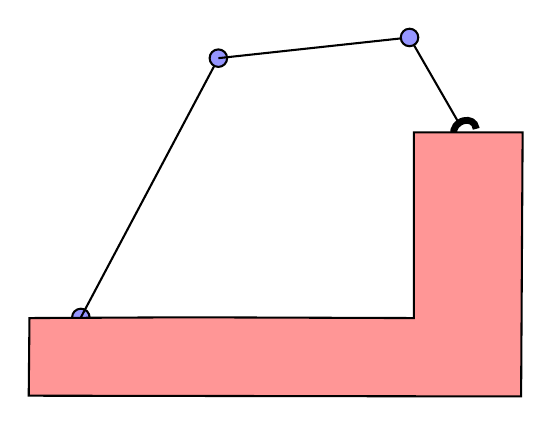
\begin{tikzpicture}[x=0.55pt,y=0.55pt,yscale=-1,xscale=1]
%uncomment if require: \path (0,300); %set diagram left start at 0, and has height of 300

%Shape: Circle [id:dp2680036705913309] 
\draw  [fill=myblue  ,fill opacity=1 ] (144.5,190.35) .. controls (144.5,187.17) and (147.07,184.6) .. (150.25,184.6) .. controls (153.43,184.6) and (156,187.17) .. (156,190.35) .. controls (156,193.53) and (153.43,196.1) .. (150.25,196.1) .. controls (147.07,196.1) and (144.5,193.53) .. (144.5,190.35) -- cycle ;
%Straight Lines [id:da511009501867824] 
\draw    (150.25,190.35) -- (240.6,20) ;
%Shape: Circle [id:dp33456176340238253] 
\draw  [fill=myblue  ,fill opacity=1 ] (234.85,20) .. controls (234.85,16.82) and (237.42,14.25) .. (240.6,14.25) .. controls (243.78,14.25) and (246.35,16.82) .. (246.35,20) .. controls (246.35,23.18) and (243.78,25.75) .. (240.6,25.75) .. controls (237.42,25.75) and (234.85,23.18) .. (234.85,20) -- cycle ;
%Straight Lines [id:da8106680503102979] 
\draw    (240.6,20) -- (366.2,6.4) ;
%Straight Lines [id:da7152287278059997] 
\draw    (399.4,64) -- (366.2,6.4) ;
%Shape: Circle [id:dp1080265764134869] 
\draw  [fill=myblue  ,fill opacity=1 ] (360.45,6.4) .. controls (360.45,3.22) and (363.02,0.65) .. (366.2,0.65) .. controls (369.38,0.65) and (371.95,3.22) .. (371.95,6.4) .. controls (371.95,9.58) and (369.38,12.15) .. (366.2,12.15) .. controls (363.02,12.15) and (360.45,9.58) .. (360.45,6.4) -- cycle ;
%Shape: Block Arc [id:dp8677516838116468] 
\draw  [fill={rgb, 255:red, 0; green, 0; blue, 0 }  ,fill opacity=1 ] (397.16,75.17) .. controls (396.21,74.66) and (395.39,73.93) .. (394.76,73.02) .. controls (392.25,69.38) and (393.66,64.05) .. (397.92,61.11) .. controls (402.18,58.16) and (407.67,58.73) .. (410.18,62.36) .. controls (410.82,63.28) and (411.2,64.3) .. (411.35,65.37) -- (408.23,66.19) .. controls (408.19,65.47) and (407.96,64.78) .. (407.55,64.18) .. controls (406.04,62) and (402.55,61.8) .. (399.74,63.74) .. controls (396.94,65.68) and (395.88,69.02) .. (397.39,71.2) .. controls (397.8,71.8) and (398.37,72.25) .. (399.02,72.54) -- cycle ;
%Shape: Polygon [id:ds12621320375323086] 
\draw  [fill=mypink  ,fill opacity=1 ] (440.5,68.75) -- (369,68.75) -- (369,190.75) -- (219.5,190.25) -- (116.5,190.75) -- (116,241.75) -- (439.5,242.25) -- cycle ;




\end{tikzpicture}

    %\caption{Caption}
    %\label{fig:my_label}
\end{figure}

\end{flushleft}
\end{frame}



\begin{frame}
\centerline{Lecture slides are available via Moodle.}
\bigskip
\centerline{You can help improve these slides at:}
\centerline{\href{https://github.com/SergeiSa/Contact-Aware-Control-Slides-Fall-2020}{github.com/SergeiSa/Contact-Aware-Control-Slides-Fall-2020}}
\bigskip
\centerline{Check Moodle for additional links, videos, textbook suggestions.}
\end{frame}

\end{document}
